\documentclass[notitlepage]{report}
\usepackage[left=1in, right=1in, top=1in, bottom=1in]{geometry}

\usepackage{titling}
\usepackage{lipsum}
\usepackage[colorlinks = true]{hyperref}
\usepackage{graphicx}
\usepackage[thinc]{esdiff}
\usepackage{matlab-prettifier}
\usepackage{listings}
\usepackage{cite}
\usepackage{amsmath,amssymb,amsfonts}
\usepackage{algorithmic}
\usepackage{graphicx}
\usepackage{textcomp}
\usepackage{xcolor}

\pretitle{\begin{center}\Huge\bfseries}
\posttitle{\par\end{center}}
\preauthor{\begin{center}\Large\ttfamily}
\postauthor{\end{center}}
\predate{\par\large\centering}
\postdate{\par}

\title{Digital Image Processing (CS7.404)\\
Assignment 0}
\author{Soham Vaishnav | 2022112002\\
soham.vaishnav@research.iiit.ac.in}
\date{\today}
\begin{document}

\maketitle

\begin{abstract}
Assignment 0 deals with fundamental image processing techniques including manipulation of color as well as 
grayscale images. The tasks range from basic ones like reading from and writing to images to converting 
grayscale images into color ones using pseudocoloring. Some of the tasks are relatively complex like 
Chroma Keying, reading from and writing into a video (essentially an array of frames) and creating a video 
wherein one image transforms into another image via a smooth transition using some special effect like fading
or sliding. The assingment entails using majorly three libraries - OpenCV, Numpy and Matplotlib. OS library has 
also been used for integrating file and directory paths and to validate their existence.
\end{abstract}

\section{Task 1 - Reading from Image}
This task involves reading an image from the folder into an array for any future use. I have used \textbf{OpenCV}
for the majority of the task.

\begin{figure}[htp]
    \centering
    \hypertarget{C1}{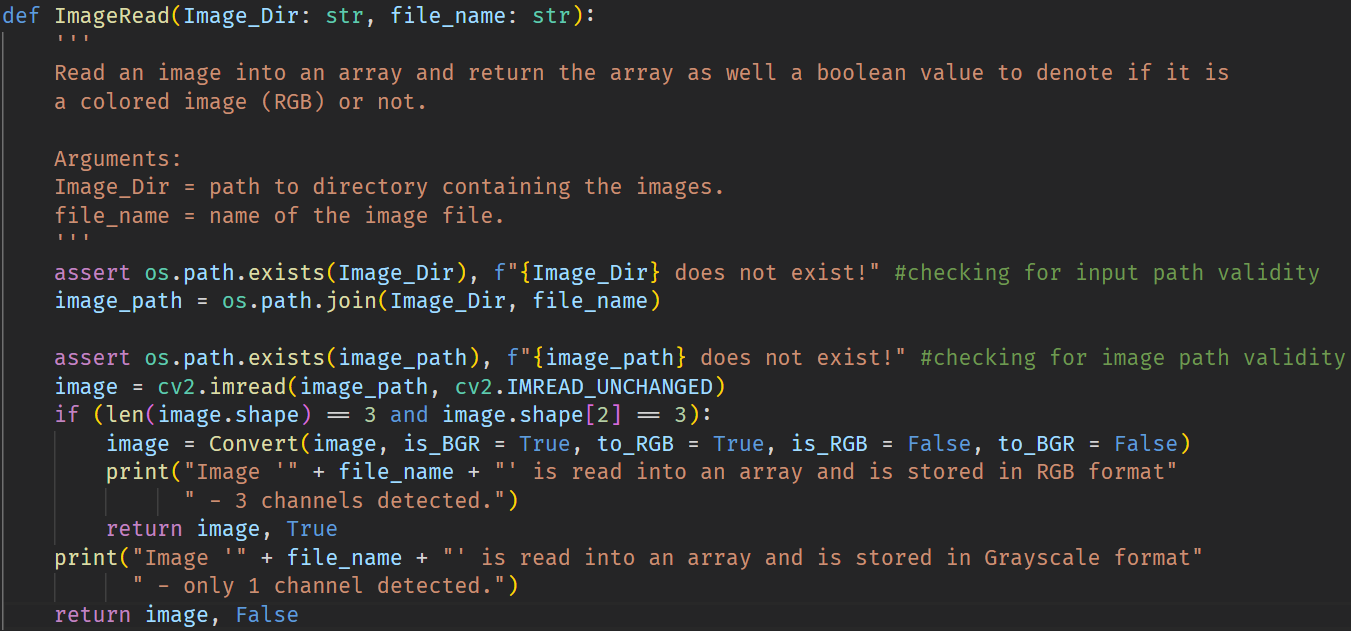
\includegraphics[width = 0.7\textwidth]{C1.png}}
    \caption{Function for reading from an image into an array}
    \label{fig1:sysfig}
\end{figure}

The inputs to the function are the image directory and the name of the image we want to read from. The function
returns the image array as well as a boolean denoting its type (color or grayscale). Note that the image returned 
is in RGB format after conversion from BGR which OpenCV returns. The outputs 
can be seen in the main jupyter book. 

\section{Task 2 - Writing to Image}  
This task involves writing an array of numbers into an image while taking care of it being grayscale
or colored. Again, OpenCV library has been used for the major part of this task. 

\begin{figure}[htp]
    \centering
    \hypertarget{C2}{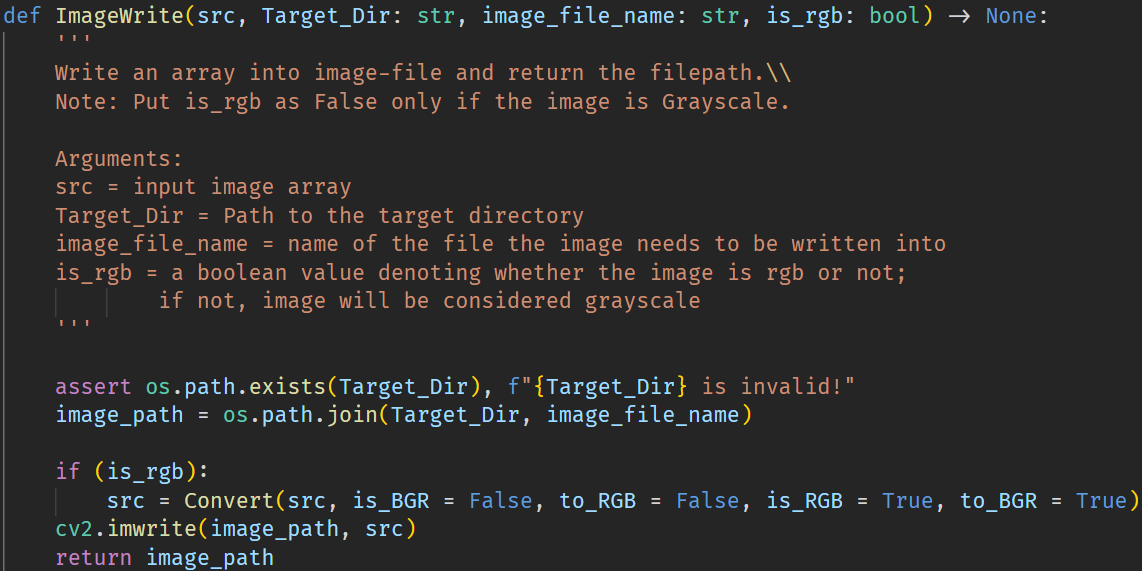
\includegraphics[width = 0.7\textwidth]{C2.png}}
    \caption{Function for writing to an image from an array}
    \label{fig2:sysfig}
\end{figure}

The inputs to the function are the source array which needs to be written to the image, target directory 
and filename along with a boolean value denoting whether the image should be RGB (if False, then the image is taken to
be grayscale - this helps in storing the image in BGR/Grascale format). The function returns the local path to the 
location of the image. Outputs can be seen in the main jupyter notebook.

\section{Task 3 - Brightness Change}
Given an image, the aim of this task is to change its brightness by some factor which will be added uniformly across the 
image. The code is designed to make this factor - \textit{b\textunderscore factor} - user defined.

\begin{center}
    $R(x, y) = S(x, y) + bf$
\end{center}

On setting various values for the brightness factor, we get a range of images with varying brightness.

\begin{figure}[htp]
    \centering
    \hypertarget{BF}{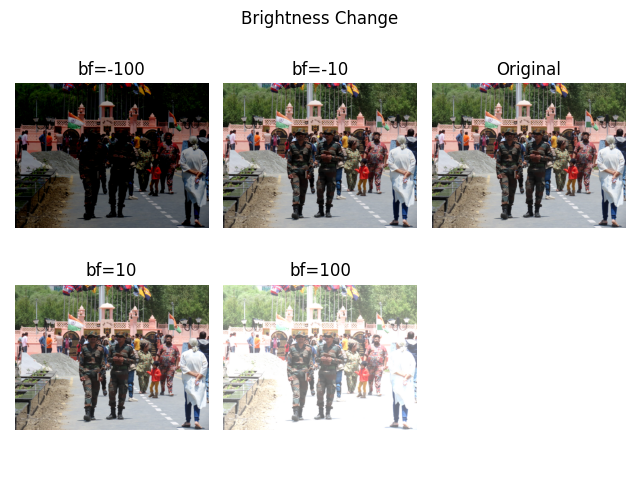
\includegraphics[width = 0.6\textwidth]{BF.png}}
    \caption{Grid of images depicting varying brightness where bf = brightness factor}
    \label{fig3:sysfig}
\end{figure}

\begin{figure}[htp]
    \centering
    \hypertarget{BF_Hist}{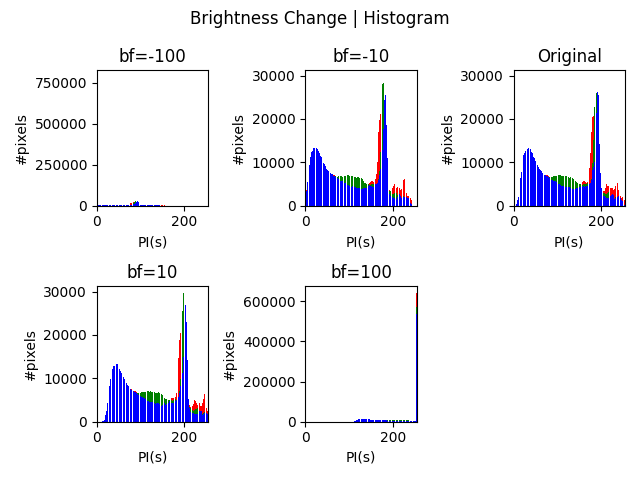
\includegraphics[width = 0.6\textwidth]{BF_Hist.png}}
    \caption{Grid of histograms depicting effects of varying brightness where bf = brightness factor and PI(s) = pixel intensities}
    \label{fig4:sysfig}
\end{figure}

The shift is evident in the histograms.
(For the histograms with bf = -100 and bf = +100, the y-range is very large and to fit it alongside other ones, 
the bars are not very clearly visible).

Code for this task has not been attached in the report but can be found along with the plots in the main code file.

\textbf{Note:} For this task, since we are adding some factor to the image to increase or decrease its brightness, the 
pixel values tend to get out of the range which makes plotting and visualising the image very difficult. To counter this, 
while adding, the pixel values are clipped to stay within range [0, 255]. Finally, the datatype of the array is converted to 
uint8 for visualisation purposes.

\section{Task 4 - Contrast Stretching}
Contrast stretching is one method to beatify an image to be able to draw as much information as possible from the image. This
technique is applied on the images which are of low-contrast. Low-constrast implies that the range of values that the pixels of 
the image takes is limited to a very small region between 0 and 255; in effect the histogram looks very skewed or shrunken to a small
region. Since all the color intensities are very near to one another the perceivable difference in the image is very less, hence low-contrast.

The aim of this task is to convert a low-contrast image into a high-contrast one. Two methods to do it:
\begin{itemize}
    \item \textbf{Linear}: Involves simply multiplying the image by a constant and then clipping for the values that go out of the 
    permissible range.
    \begin{center}
        $R(x, y) = \alpha S(x, y)$
    \end{center}
    \item \textbf{Non-Linear}: Involves piece-wise stretching of the pixel values. Here, for each short range (three) of 
    permissible values (0 to 255) a separate function is defined for performing the stretching.
\end{itemize}
\newpage

\begin{figure}[htp]
    \centering
    \hypertarget{CStretch_ref}{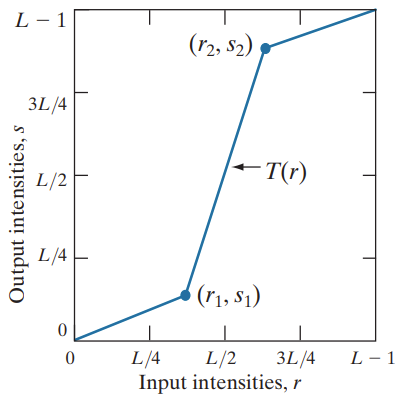
\includegraphics[width = 0.2\textwidth]{CStretch_ref.png}}
    \caption{Formulation of piece-wise contrast stretching - taken from Digital Image Processing textbook}
    \label{fig5:sysfig}
\end{figure}

The code I wrote gives the user to choose any of the above methods to do contrast stretching. It also, infact allows the user
to perform \textbf{contrast compression} (reverse of contrast stretching). The results I show are of an image which has been 
converted to a low-constrast one and then changed back to stretched version using constrast stretching. The image for non-linear
method is on the next page (Figure.7).

\begin{figure}[htp]
    \centering
    \hypertarget{CStretch_Lin}{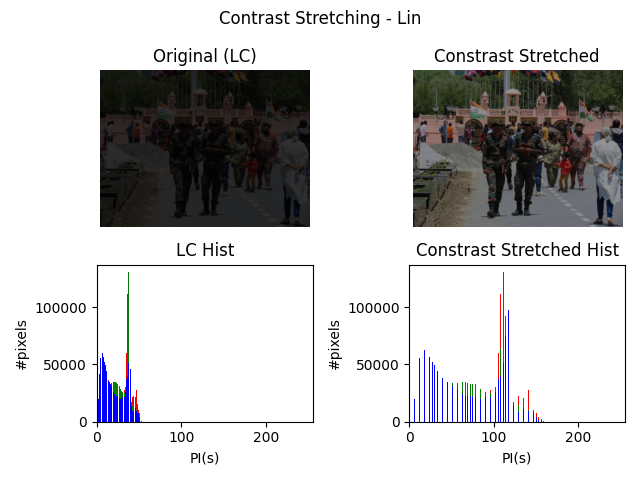
\includegraphics[width = 0.6\textwidth]{CStretch_L.png}}
    \caption{Contrast Stretching using Linear method}
    \label{fig6:sysfig}
\end{figure}

\begin{figure}[htp]
    \centering
    \hypertarget{CStretch_Lin}{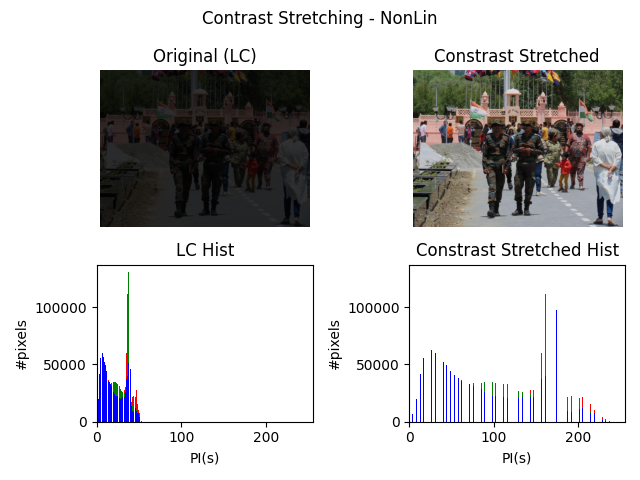
\includegraphics[width = 0.6\textwidth]{CStretch_NL.png}}
    \caption{Contrast Stretching using Non-Linear method}
    \label{fig7:sysfig}
\end{figure}

\section{Task 5 - Color to Grayscale}
This task involves converting the image space of an image - taking it from RGB space to Grayscale space. One major change
that is seen here, and which is quite natural, is that the number of channels decrease from 3 (in case of RGB) to 1 (in Grayscale).
This also implies that the grayscale image occupies less memory than its coloured counterpart. Now, although the number of channels has
decreased, the range of values that the pixels can take still remains the same (i.e., 0 to 255). A few methods to do this:
\begin{itemize}
    \item \textbf{Luminance-based}: Uses the colorimetry principles and the considers biological sensitivity of the human eye 
    in perceiving R, G and B channels. This method preserves the luminance aspect of the image (light directions, etc.) and therefore
    looks natural. The weights associated with R, G and B channels here are 0.2126, 0.7152 and 0.0722 respectively. (ref.: Wikipedia).
    \item \textbf{Arithmetic Mean-based}: A very straightforward method taking mean of all the three channel pixel values and that mean 
    becomes the grayscale pixel value.
    \item \textbf{Max-of-all -based}: Here we take the maximum of the three channel values for each pixel in the color image and this value
    then becomes the resultant gray value. Renders an image more towards the brighter end of the spectrum.
    \item \textbf{Min-of-all -based}: Similar to max-of-all method, here we take the minimum. Renders an image more towards the darker end of the
    spectrum.
    \item \textbf{Desaturation-based}: Here we use the max-of-all and min-of-all methods to find the arithmetic mean of both and give that
    value to our grayscale image.
    \item \textbf{Weighted Average-based}: Here we put any arbitrary weights to R, G and B channels and see the effects (I have made this
    user-defined inputs).
\end{itemize}

\begin{figure}[htp]
    \centering
    \hypertarget{C2G}{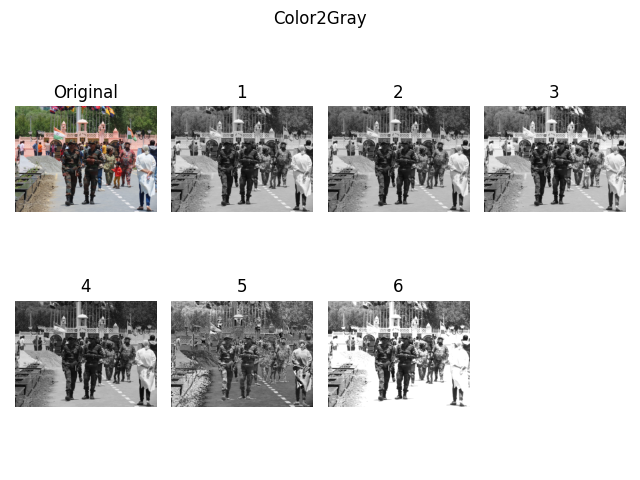
\includegraphics[width = 0.6\textwidth]{C2G.png}}
    \caption{Color to Grayscale using the six methods listed above (in the same order)}
    \label{fig8:sysfig}
\end{figure}

\begin{figure}[htp]
    \centering
    \hypertarget{C2G_Hist}{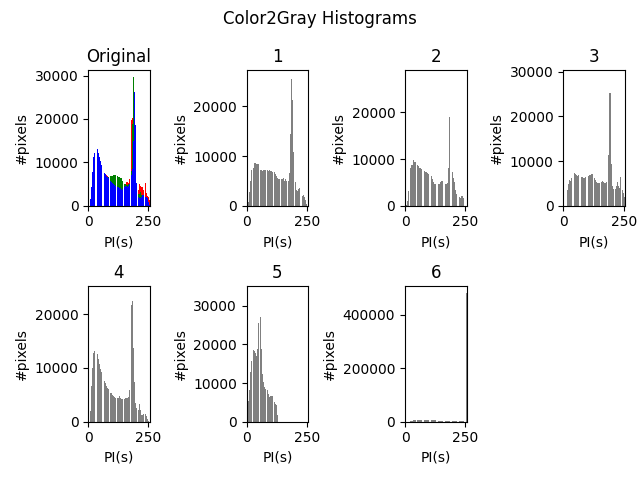
\includegraphics[width = 0.6\textwidth]{C2G_Hist.png}}
    \caption{Histograms for color to grayscale using the six methods listed above (in the same order)}
    \label{fig9:sysfig}
\end{figure}

\section{Task 6 - Grayscale to Color}
This was a tricky task but interesting because there was no right answer to it (ofcourse except the actual image) and thus, a lot of 
space for experimentation was there. I made use of, as was mentioned, pseudo-coloring to generate colors for a grayscale image. The method
I thought of was quite straight forward and involved making gradients for the three primary colors (R, G and B in our case) using fading techniques.
For instance, I started off with Blue, then while it was gradually set to fade, I was proportionally increasing Green. Then for the next part of
the gradient, I started to fade Green and gradually pushed Red into picture finally culminating in a dark or bright tone. I generated the following 
gradients:

\begin{figure}[htp]
    \centering
    \hypertarget{Grads}{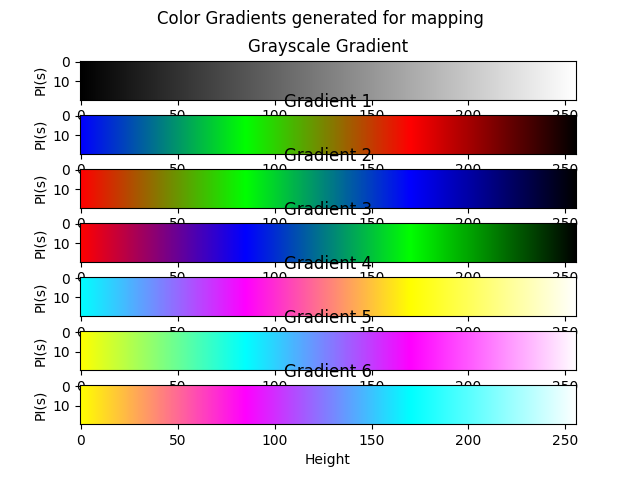
\includegraphics[width = 0.6\textwidth]{Grads.png}}
    \caption{Color Gradients generated for pseudo-color mapping}
    \label{fig10:sysfig}
\end{figure}

The gradient-wise images are as follows:

\begin{figure}[htp]
    \centering
    \hypertarget{G2C}{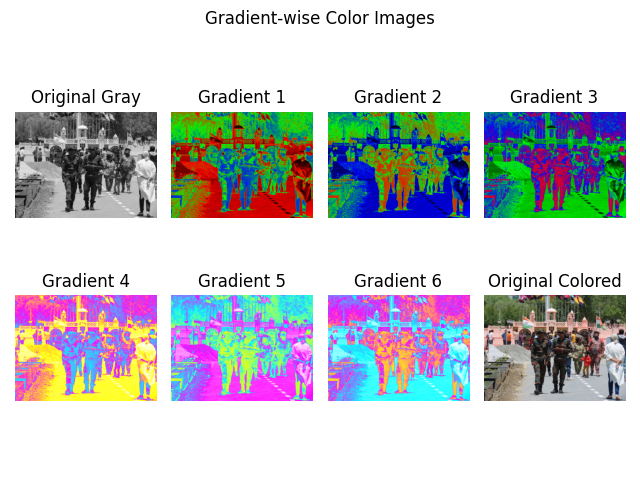
\includegraphics[width = 0.7\textwidth]{G2C.png}}
    \caption{Color Gradients-based color Images}
    \label{fig11:sysfig}
\end{figure}

And some extras...
\begin{figure}[htp]
    \centering
    \hypertarget{Grads}{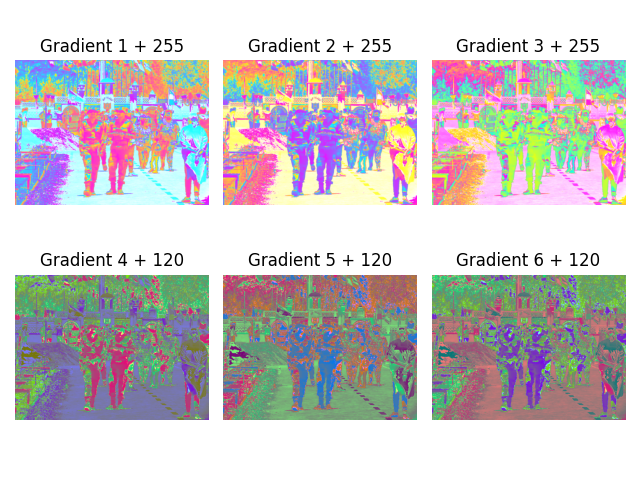
\includegraphics[width = 0.7\textwidth]{G2C_extras.png}}
    \caption{Some extra images obtained after playing around with the ones in Figure.11}
    \label{fig12:sysfig}
\end{figure}

\textbf{Note:} Clipping was required in all the above generated color images.

\section{Task 7 - Chroma Keying}
Chroma keying is the name given to the process of removing greenscreen background from an image and replacing 
it with any other background that one wants. Therefore, this at least needs 2 images to start with - one foreground (with greenscreen) 
and the background (which will replace the greenscreen).

It is quite clear that to remove the background, we first need to know the numeric distribution of the pixel intensities in both the images, 
and what better than a histogram to do it.
I used the following images:

\begin{figure}[htp]
    \centering
    \hypertarget{CK}{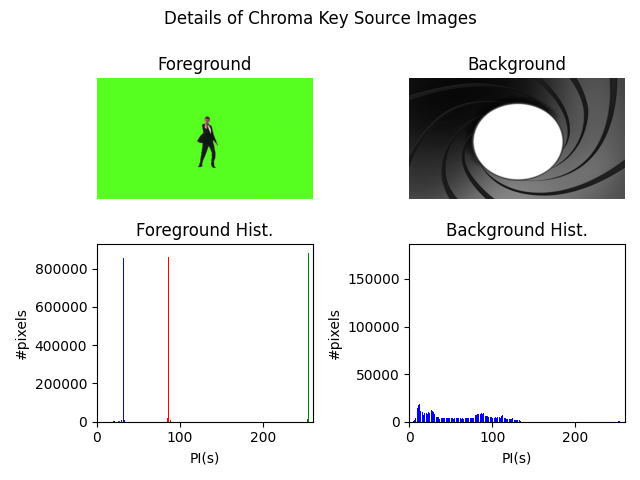
\includegraphics[width = 0.6\textwidth]{CK.png}}
    \caption{Chroma Keying input images}
    \label{fig13:sysfig}
\end{figure}

As we can see in the images, the green pixel count of foreground image is quite high and almost completely towards the lighter end
of the spectrum. In my method, I conveniently removed the pixels with values above 210, and superimposed the background over it to get the required
effects. The method looks as follows:

\begin{figure}[htp]
    \centering
    \hypertarget{C7}{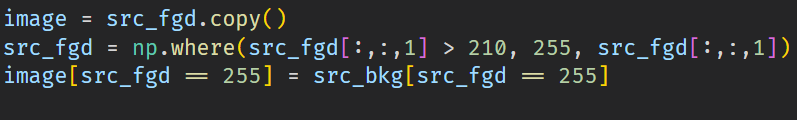
\includegraphics[width = 0.6\textwidth]{C7.png}}
    \caption{Chroma Keying algorithm}
    \label{fig14:sysfig}
\end{figure}

The algorithm commented out as \textit{Aliter} also does the same work but is implemented using \textbf{for-loops} whereas, 
the one which isn't commented out is the vectorised version of the same thing.

On doing this, I get the final image which looks as shown below:

\begin{figure}[htp]
    \centering
    \hypertarget{CK_out}{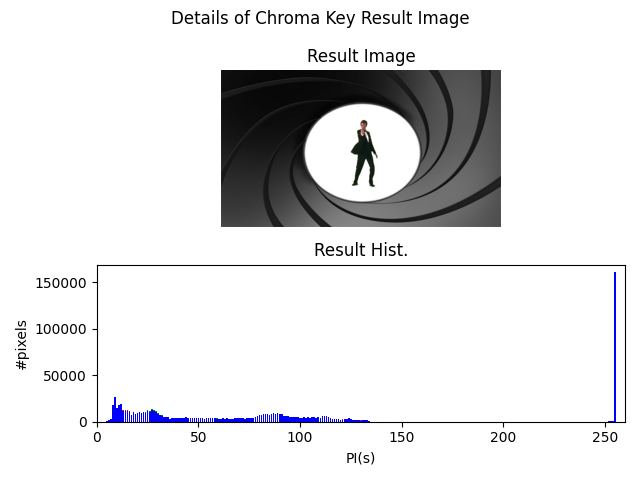
\includegraphics[width = 0.6\textwidth]{CK_out.png}}
    \caption{Chroma Keying output image}
    \label{fig15:sysfig}
\end{figure}

\begin{figure}[htp]
    \centering
    \hypertarget{CK_out}{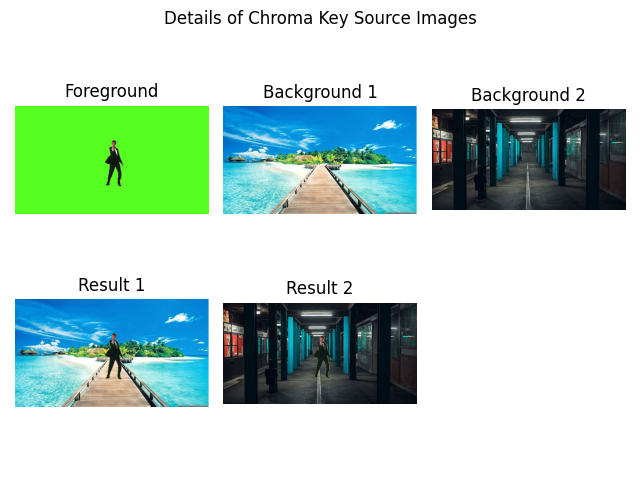
\includegraphics[width = 0.6\textwidth]{CK_Extras.png}}
    \caption{Some other trials with the same foreground but different \textit{suitable} backgrounds}
    \label{fig16:sysfig}
\end{figure}

\textbf{Note:} The function has the ability to take care of images with unequal shapes (H and W values). For this
the function makes use of the \textbf{Resize} functionality of OpenCV (a one line code).

\section{Task 8 - Reading from and Writing to a Video}
Videos are essentially nothing but a sequence of frames (images) being rapidly changed by sampling time. The rate at which the frames move (FPS)
and the duration of the video determine the number of frames that the video includes. Taking into consideration the persistance of vision which is around
$\frac{1}{16}^{th}$ of a second, that is, 16 frames per second, any FPS above that should be fine. 

To carry this task out, I made use of OpenCV functions that help one in reading and writing into images; specifically, I used \textbf{VideoCapture} and
\textbf{VideoWriter} to do the reading from and writing to tasks respectively.

While reading the video, I stored the images - as arrays - in a concatenated form as a list. This was for three reasons - one, to not occupy memory
in the machine, second, to sustain the sequence and third, for easier access across various other functions (such as writing or editing).
While writing to the video, I accessed the stored frames - as arrays - in a sequential manner. I have kept FPS as well as the codec as a user-defined variable 
for one to play around with (in case of FPS) and to select the right video extension (in case of codec). 

\textbf{Learning:} There was one major learning worth mentioning separately while writing to a video which was to realise that OpenCV
understands the image in WHC (weight, height and channels) format when it comes to giving these params as inputs. It took me a while to 
figure out this since I was giving the frames in HWC format which kept on shooting errors. The original video is 
\href{https://iiitaphyd-my.sharepoint.com/:v:/g/personal/soham_vaishnav_research_iiit_ac_in/Ec_j7y3V879EngubQkT_wU4BXeToZQwFjUkFBHgawnIIsA?nav=eyJyZWZlcnJhbEluZm8iOnsicmVmZXJyYWxBcHAiOiJPbmVEcml2ZUZvckJ1c2luZXNzIiwicmVmZXJyYWxBcHBQbGF0Zm9ybSI6IldlYiIsInJlZmVycmFsTW9kZSI6InZpZXciLCJyZWZlcnJhbFZpZXciOiJNeUZpbGVzTGlua0NvcHkifX0&e=qzGjbD}{here}
and the link to the recreated video can be found 
\href{https://iiitaphyd-my.sharepoint.com/:v:/g/personal/soham_vaishnav_research_iiit_ac_in/EY-A4Kj5dd9Kqraze4W-jf0BFBeDbjO1vpnLBdHrQsBkiA?nav=eyJyZWZlcnJhbEluZm8iOnsicmVmZXJyYWxBcHAiOiJPbmVEcml2ZUZvckJ1c2luZXNzIiwicmVmZXJyYWxBcHBQbGF0Zm9ybSI6IldlYiIsInJlZmVycmFsTW9kZSI6InZpZXciLCJyZWZlcnJhbFZpZXciOiJNeUZpbGVzTGlua0NvcHkifX0&e=RPeIJL}{here}.

\textbf{Note:} The input video file has to contain all frames in colored format.

\section{Task 9 - Creating a Special-Effects Video}
This was one the most interesting tasks which involved using some special effect such as fading, sliding or any other had to be used to make a video wherein one image
makes a transition into another. I wrote a function facilitating one to play around with either of the effects (with custom duration and FPS) using the following techniques:
\begin{itemize}
    \item \textbf{Fade:} Using the input FPS and duration, I calculate the number of frames that the video will have and then iterate over that number to generate those frames
    using the formula:
    \begin{center}
        $R(n) = (1-\frac{n}{N})S_1 + (\frac{n}{N})S_2$
    \end{center}
    where $S_1$ and $S_2$ are source images, N is the total number of frames and n is the iteration variable which goes from 0 to N-1.
    \item \textbf{Slide:} Here I did not make use of FPS in determing the number of frames as by choosing this effect the function automatically selects the 
    total number of frames to be equal to the columns of one of the images. This is because the driving logic for this effect is to copy the new image column-by-column
    over the first image thereby creating a \textit{sliding} effect. 
\end{itemize}

Outputs videos can be found here:
\begin{itemize}
    \item \href{https://iiitaphyd-my.sharepoint.com/:v:/g/personal/soham_vaishnav_research_iiit_ac_in/ETZDCFDibwJPpaSgd_yHo3EBmKhZDK9ihggEEYdAYTPnCA?nav=eyJyZWZlcnJhbEluZm8iOnsicmVmZXJyYWxBcHAiOiJPbmVEcml2ZUZvckJ1c2luZXNzIiwicmVmZXJyYWxBcHBQbGF0Zm9ybSI6IldlYiIsInJlZmVycmFsTW9kZSI6InZpZXciLCJyZWZlcnJhbFZpZXciOiJNeUZpbGVzTGlua0NvcHkifX0&e=viOq7r}{Fade}
    \item \href{https://iiitaphyd-my.sharepoint.com/:v:/g/personal/soham_vaishnav_research_iiit_ac_in/EZKr7tYxMEpDqLKFYQYEAkIB3AHYE3ZuQwMCcb82G2IdiQ?nav=eyJyZWZlcnJhbEluZm8iOnsicmVmZXJyYWxBcHAiOiJPbmVEcml2ZUZvckJ1c2luZXNzIiwicmVmZXJyYWxBcHBQbGF0Zm9ybSI6IldlYiIsInJlZmVycmFsTW9kZSI6InZpZXciLCJyZWZlcnJhbFZpZXciOiJNeUZpbGVzTGlua0NvcHkifX0&e=yLP1Lg}{Slide}
\end{itemize}

\begin{figure}[htp]
    \centering
    \hypertarget{T9_in}{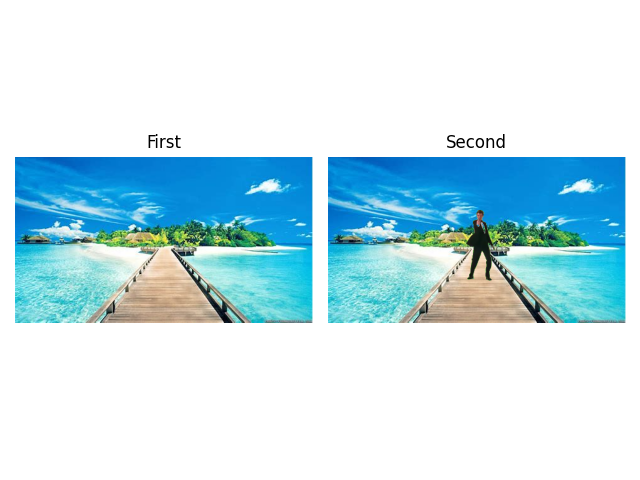
\includegraphics[width = 0.6\textwidth]{T9_in.png}}
    \caption{Input images to Task 9}
    \label{fig17:sysfig}
\end{figure}

Few things to \textbf{note}: The shape of both the images has to be equal otherwise these effects will not work. But, the user does not need to worry about this! The function for 
this task will take care of the unequal shapes by detecting it and employing the \textbf{Resize} functionality of OpenCV. One thing that the one does need to take care about while
putting in inputs is that the function will not accept 2 different \textit{types} of images - color and grayscale; either both have to be color or both need to be grayscale. 

\section{Misc. Functions}
I created some miscellaneous or helper functions that make some tasks easier:
\begin{itemize}
    \item \textbf{Generate Histograms:} I wrote a function that takes an image and its type as an input and generates appropriate histogram for it. Simply
    calling this function during visualisation saves some repetitive lines of code!
    \item \textbf{Convert:} I wrote this function which aims to convert the type of image from BGR to RGB and vice-versa. Although only 3 lines of code, this comes a lot in handy 
    when we realise that to visualise an image using Matplotlib which has been read using OpenCV, conversion is very necessary. This is because OpenCV reads an image in BGR format 
    and Matplotlib visualises it using RGB format, thereby rendering a very weird image as an output.
\end{itemize}

Finally, as a \textbf{note}, all the task has been majorly carried out using just Numpy and Matplotlib. OpenCV has only been used for tasks such as reading, writing or resizing.

\end{document}